\section{Überblick}

\subsection{Schach und KI}

% ================================================================================ %
\begin{frame}{Schach und KI}
\begin{itemize}
	\item Eines der am längsten erforschten Teilgebiete der KI
	\item Häufig Forschung in Bezug auf Schach Engines
	\begin{itemize}
		\item Ziel ist die Optimierung der Spielstärke eines Schachprogramms
		\item Spielstärke von Engines liegt weit über der von Menschen
	\end{itemize}
	\item Professionelle Schachspieler oder Kommentatoren werden benötigt um Absicht hinter Zügen zu verstehen
	\item Problem: Züge werden nicht immer richtig verstanden
\end{itemize}
\end{frame}
% ================================================================================ %

\subsection{Forschungsfrage}

% ================================================================================ %
\begin{frame}{Forschungsfrage}
\begin{center}
\begin{large}
\textit{Wie kann maschinelles Lernen genutzt werden,\\um Kommentare zu Schachpartien zu generieren?}
\end{large}
\end{center}
\end{frame}
% ================================================================================ %

\subsection{Aufbau}

% ================================================================================ %
\begin{frame}{Aufbau}
\begin{itemize}
	\item Der Prozess der Kommentarerzeugung wird in zwei Teile aufgeteilt
	\begin{itemize}
		\item Bereitstellung von Informationen (Schach Engine)
		\begin{itemize}
			\item Computerverständliche Schachbrettdarstellung
			\item Zugsuche
			\item Positionsbewertung
		\end{itemize}
		\item Generierung von Kommentaren (Virtueller Schachkommentator)
		\begin{itemize}
			\item Festlegen was man übersetzen möchte
			\item Architektur zur Erzeugung von Schachkommentaren
		\end{itemize}
	\end{itemize}
\end{itemize}
\begin{figure}
\centering
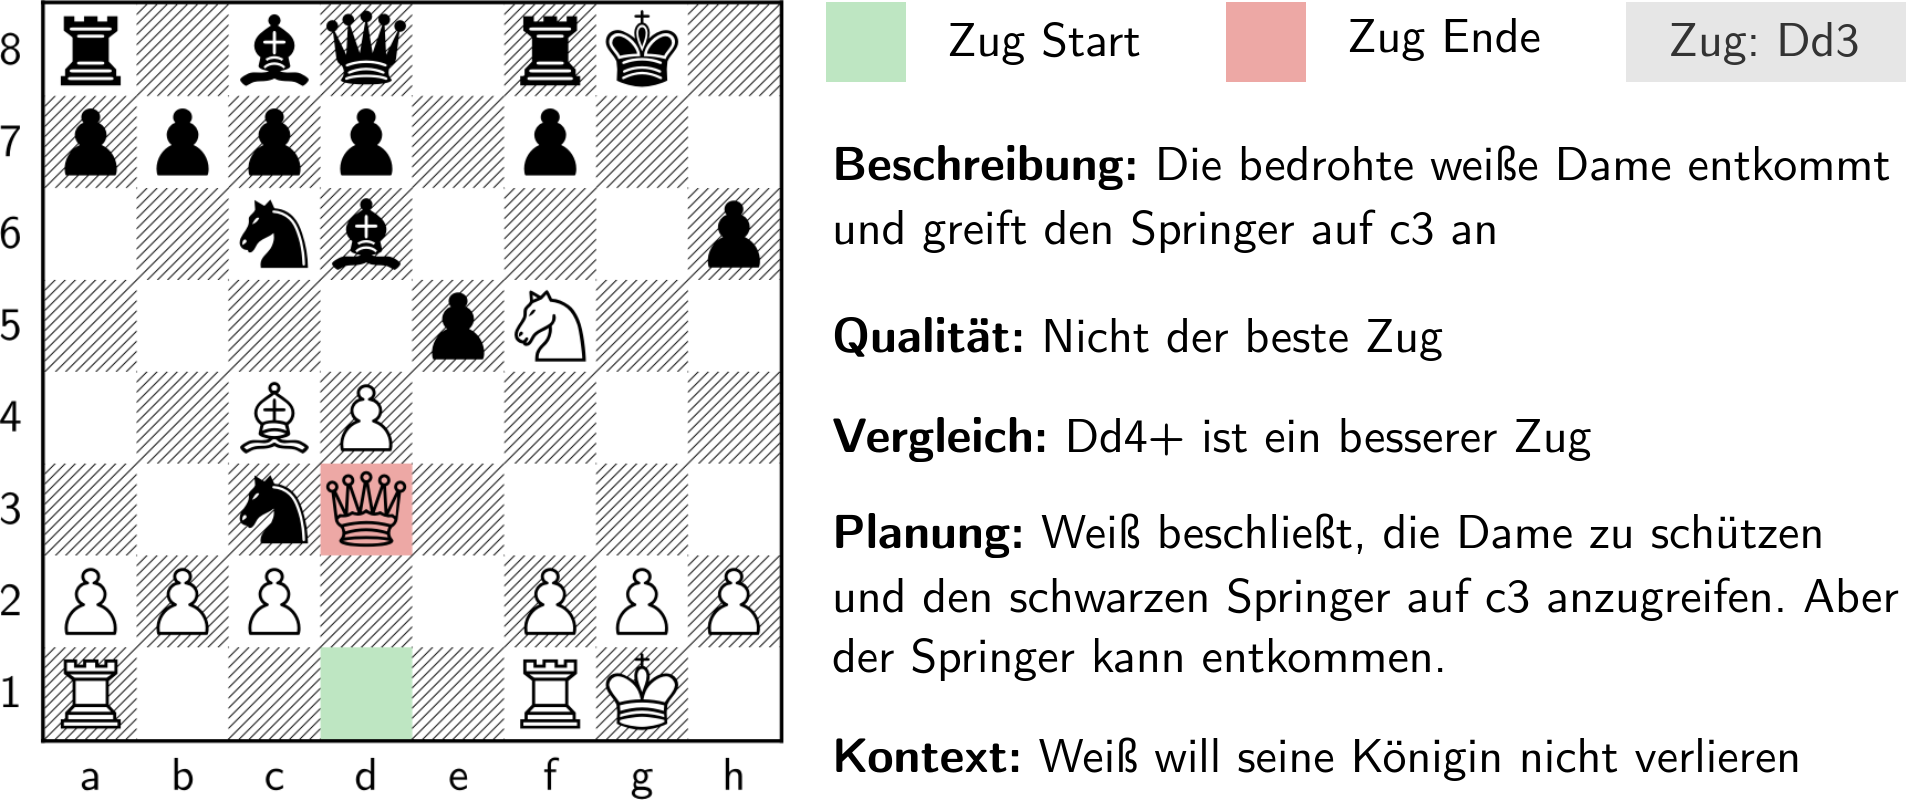
\includegraphics[width=0.55\textwidth]{graphics/commentator_example/commentator.png}
\end{figure}
\end{frame}
% ================================================================================ %